\documentclass{article}
\usepackage[utf8]{inputenc}
\usepackage[dvipsnames]{xcolor}
\usepackage{amsmath, amsthm, amssymb, amscd, amsxtra,color,authblk,tikz,arydshln,array, caption, romannum,verbatim,enumitem}
\usetikzlibrary{shapes,arrows,positioning}
\usepackage[T1]{fontenc}
\usetikzlibrary{decorations.markings}

\begin{document}

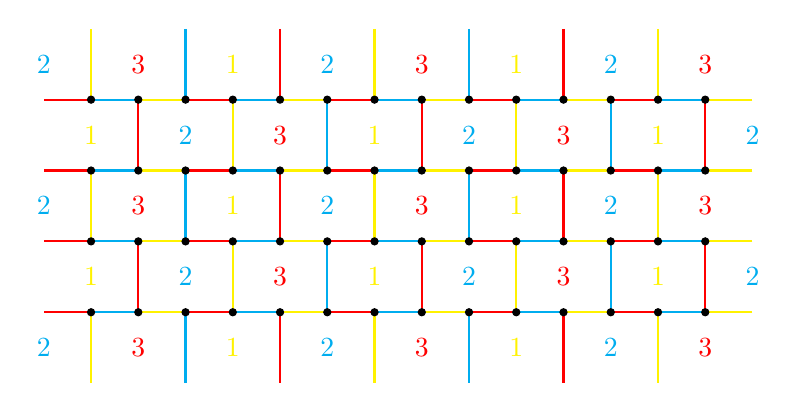
\begin{tikzpicture}[scale=0.3]
\foreach \i in {2,14,26}
\foreach \j in {3,9,15}
        \draw[thick, yellow] ({\i},{\j}) -- ({\i},{\j-3});
\foreach \i in {6,18}
\foreach \j in {3,9,15}
        \draw[thick, cyan] ({\i},{\j}) -- ({\i},{\j-3});
\foreach \i in {10,22}
\foreach \j in {3,9,15}
        \draw[thick, red] ({\i},{\j}) -- ({\i},{\j-3});
\foreach \i in {4,16,28}
\foreach \j in {6,12}
        \draw[thick, red] ({\i},{\j}) -- ({\i},{\j-3});
\foreach \i in {8,20}
\foreach \j in {6,12}
        \draw[thick, yellow] ({\i},{\j}) -- ({\i},{\j-3});
\foreach \i in {12,24}
\foreach \j in {6,12}
        \draw[thick, cyan] ({\i},{\j}) -- ({\i},{\j-3});
\foreach \i in {2,8,14,20,26}
\foreach \j in {3,6,9,12}
        \draw[thick, red] ({\i},{\j}) -- ({\i-2},{\j});
\foreach \i in {4,10,16,22,28}
\foreach \j in {3,6,9,12}
        \draw[thick, cyan] ({\i},{\j}) -- ({\i-2},{\j});
\foreach \i in {6,12,18,24,30}
\foreach \j in {3,6,9,12}
        \draw[thick, yellow] ({\i},{\j}) -- ({\i-2},{\j});

\foreach \i in {2,6,10,14,18,22,26}
\foreach \j in {3,6,9,12}
        \filldraw[black] ({\i},{\j}) circle (0.15);
\foreach \i in {4,8,12,16,20,24,28}
\foreach \j in {3,6,9,12}
        \filldraw[black] ({\i},{\j}) circle (0.15);
\foreach \i in {8,20}
\foreach \j in {1.5,7.5,13.5}
        \node[yellow] at ({\i},{\j}) {$1$};
\foreach \i in {2,14,26}
\foreach \j in {4.5,10.5}
        \node[yellow] at ({\i},{\j}) {$1$};
\foreach \i in {0,12,24}
\foreach \j in {1.5,7.5,13.5}
        \node[cyan] at ({\i},{\j}) {$2$};
\foreach \i in {6,18,30}
\foreach \j in {4.5,10.5}
        \node[cyan] at ({\i},{\j}) {$2$};
\foreach \i in {4,16,28}
\foreach \j in {1.5,7.5,13.5}
        \node[red] at ({\i},{\j}) {$3$};
\foreach \i in {10,22}
\foreach \j in {4.5,10.5}
        \node[red] at ({\i},{\j}) {$3$};
\end{tikzpicture}

\end{document}